\DailyTitle{6265 Log (October 1, 2010)}

\DailySection{Goals}

\begin{enumerate}
\item Check the opposite-sign dimuon spectrum and note anything interesting, especially the ``muonium'' peak.
\item How does the trigger prescale work?
\item Sort out the purpose of Hcal noiseline and how/what to implement
\item Summarize work on noise characterization so far
\item Make a list of to-do items on candle note
\item How to do the fit on Z shape?
\end{enumerate}

\DailySection{Summary List}

\begin{enumerate}
\item Noiseline meeting.  Not too productive without a clear-cut goal.
\item Checked quickly opposite-sign di-muon mass spectrum.
\end{enumerate}

\DailySection{Opposite-sign dimuon (global) spectrum}

The result of almost all data is shown in figure \ref{Figure_6265DiGlobalOppositeMuonMass_DataAllExceptLast}.
I still need to think about the overall underlying shape of the curve.  For example, what is the wide bump around 2 GeV and 14 GeV.
The resonances are nice however.  The tail also bends after the Z peak.

\begin{figure*}
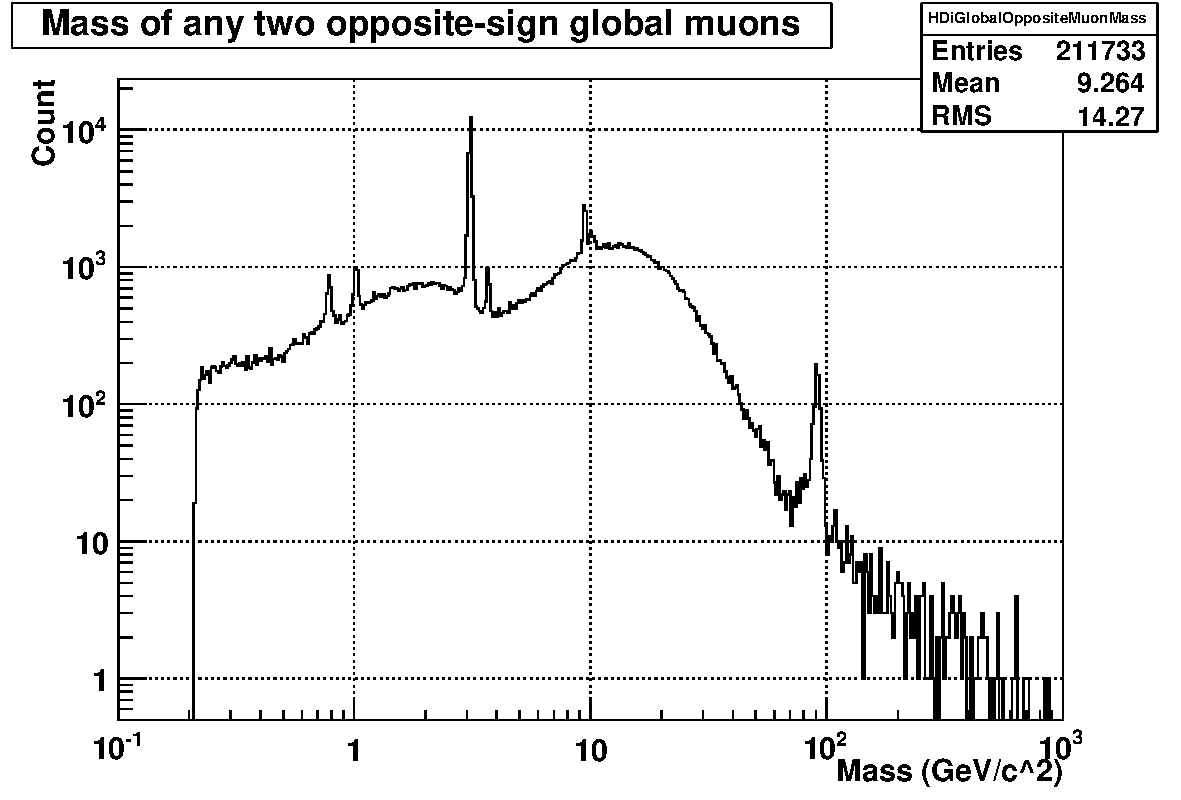
\includegraphics[width=120mm]{DailyLog/6265/6265DiGlobalOppositeMuonMass_DataAllExceptLast.pdf}
\caption{Opposite-sign dimuon (global) mass spectrum for almost full statistics (full = 2.66/pb).  The last job is
still running, and I don't think it matters for this.  The muonium peak goes away, which is nice.}
\label{Figure_6265DiGlobalOppositeMuonMass_DataAllExceptLast}
\end{figure*}

\DailySection{Work so far on noise characterization}

\DailySubSection{Things tried}

\begin{enumerate}
\item First three TS should be compatible to zero.
\item The maximum N continuous time slices.  Generalization of E2.
\item Number of time slices required to achieve P\%.  Useful to pick out sharp noise and broad noise.
\item RMS vs. mean of the 10 TS.
\item Linear fit of the pulse shape.  Potentially useful to pick out flat pulses.
\item Two-step fit.
\end{enumerate}

\DailySubSection{Late pulses - produced at interaction}

Skimmed through PDG tables and estimate what might be late, and how much energy they will deposit.
Assume distance to go is 1.4m.  See table \ref{Table_6265ParticlesMaximumDelay140cm} for numbers.

\begin{center}
\begin{table}
\begin{tabular}{|c|c|c|c|c|c|c|}
\hline
Particle & Mass (GeV) & $\tau$ (ns) & min($\beta$) & max delay (ns) & Energy (GeV) \\
\hline
$\pi+$ & 0.13957 & 26.033 & 0.176 & 26.45 & 0.142 \\
$K+$ & 0.493677 & 12.38 & 0.353 & 13.23 & 0.528 \\
$K_{0L}$ & 0.497614 & 51.16 & 0.0908 & 51.37 & 0.500 \\
p & 0.938 & $\infty$ & 0.000 & $\infty$ & 0.938 \\
n & 0.940 & $\infty$ & 0.000 & $\infty$ & 0.940 \\
$\Omega-$ & 1.67245 & 0.0821 & 0.9998 & 4.667 & 95.08 \\
$\Xi_0$ & 1.31486 & 0.29 & 0.998 & 4.676 & 21.20 \\
$\Xi_-$ & 1.32171 & 0.1639 & 0.9994 & 4.670 & 37.656 \\
\hline
\end{tabular}
\caption{Table for maximum delay (constrained by particle lifetime) of particles produced at interaction point and travelled 1.4 m.
The ``maximum delay'' is calculated using the mean lifetime.  Other particles decay too quickly, the delay would be tiny.}
\label{Table_6265ParticlesMaximumDelay140cm}
\end{table}
\end{center}

Out of these, only $\pi+$, $K+$, $K_{0L}$, proton and neutron have the chance to reach 1.4m at 12.5 ns or more.
The equivalent energy deposited would be 0.15, 0.53, 0.54, 1.01, 1.01 GeV, respectively.
Longer time delay means smaller energy - these are the ballpark numbers we expect.
If the allowed length is 3m, then the energy deposited will be 0.23, 0.82, 0.83, 1.56, 1.57 GeV.
So from the slow (relatively) stable particles produced at interaction
we expect O(1 GeV) energy deposit at most, if they were half TS or more late.

\DailySubSection{Late pulses - decay-in-flight}

The idea here is that there might be some heavy stuff produced at small $\beta$, and decay after a while to light, energetic particles.
Lab frame lifetime is $\gamma \tau$, and let's take an assumption that the decay product is extremely energetic, ie, $\beta \sim 1$.
Let's do the calculation when the parent particle stays on average 12.5 ns in lab frame, and the minimum required energy of it.

\begin{eqnarray}
T &=& 12.5 ns\nonumber\\
\gamma &=& \dfrac{T}{\tau}\nonumber\\
\beta &=& \sqrt{1 - \gamma^{-2}} = \sqrt{1 - \dfrac{\tau^2}{T^2}}\nonumber\\
\text{Distance travelled} &=& \beta \gamma c \tau = \beta c T = \beta \times 3.74 m\nonumber
\end{eqnarray}

Unless $\tau$ is close enough to $T$, the particle won't stay in the detector for 12.5 ns.  Which means that under the assumption that
the decay product is relativistic, decay-in-flight particles will at most deposit same order of energy as the ones produced at production.
If the decay product has classical velocity, it won't deposit much energy anyways.

\DailySubSection{Other items - moved to next work day to think about}

After the afternoon noiseline meeting, it seems that I have a lot on my plate already.  Let me make a definite plan on how to tackle each of them first....

\begin{enumerate}
\item Late pulses - late hadronic/EM shower-developement....what's the typical shower develop time?  What's the chance that a shower fragment makes an ion-feedback noise?
\item Out-of-time pulses - radiation from other sub-detectors...how is the strength of radiation related to dosage history (for different material)?  What's the expected dosage for certain
instantaneous luminosity?  Can we estimate the radiation from the environment?  What's the radiation content?  Mostly photons?  How about hadrons?
\item Out-of-time pulses - beam background
\item Out-of-time pulses - cosmic muons
\item Things that might worth trying
\end{enumerate}

\DailySection{Meeting notes}

\DailySubSection{6265 Morning Noiseline Meeting}

\begin{enumerate}
\item Maria had a car accident.  I hope it's not too serious.
\item The main thing to clarify is the purpose of the noiseline.  Everything goes from there.
\item Adi mentioned a few possible use cases:
   \begin{enumerate}
   \item Find noise that won't be caught otherwise
   \item Correlation between detectors (more like DQM plots)
   \item Radiation damage?
   \end{enumerate}
\item What I want is some kind of noise trend monitoring, finer than the current ion/HPD/RBX categories
\item To begin with, Artur will send me examples of DQM codes so that I can play with it.
\end{enumerate}

\DailySubSection{6265 Afternoon Noiseline Meeting}

\begin{enumerate}
\item Until we have the first result, the noiseline should be the same as exotica hotline - keep events so that we can look at it.
We want to integrate into DQM and P5 event display.
\item Have one firework display that constantly show noises + physics.  (And one for normal events, one for exotica hotline.)
\item Eventually it will become a skim.
\item To start with, we should see what is meaningful.  Find noise overlapping with physics signature (muons, etc.).
\item Artur: integrate into Hcal DQM?
\item JetMET?  Homework for Artur?
\item What is Muon DPG doing?  Homework for Piotr.
\item Now we should put whatever we have in (HCAL, ECAL).
\item Maria: We need to think about the workflow to rereco without noise cleaning.
\item How to catch new forms of noise?
\item Piotr will show dimuon results!  He will check noise in muon system and report.
\item Exotica hotline spots possible types of new noise, and we follow up on them.
\item Integrate Shuichi's monitoring to DQM?
\item Run first on exotica hotline files and see how many we keep.
\item As a first step, try to run the exotica hotline workflow.
\item Aim to have a prototype in the next two weeks.
\item Artur wants to have Hcal noise DQM done in the next two weeks.  (Attack for bonus point!)
\end{enumerate}

\DailySection{To-do's for next week}

\DailySubSection{Z+Jet Candle}

\begin{enumerate}
\item Find Matthias and update on the status of fit...strategy, etc.
\item Find out how to constrain \texttt{RooFormulaVar} to be greater than zero.
\item Check out a copy of the Z candle note and make a list of items to produce (and automize).
\item Check with Maurizio and see if I miss anything.
\end{enumerate}

\DailySubSection{W+Jet Fit Without b-tagging}

\begin{enumerate}
\item Check with Chris to discuss on the strategy.  Maybe there is a working fit from electrons.
\end{enumerate}

\DailySubSection{Hcal Noise Characterization}

\begin{enumerate}
\item Continue doing subtraction from noise sample.
\item Make a signal root file and see where the signal lands.
\item Get the most recent timing correction from Jeremy et. al.
\item Condense into a few categories of noise shape and make \texttt{EDFilter} of them.
\item Then it's ripe to integrate into DQM
\end{enumerate}

\DailySubSection{Hcal Noiseline Project}

\begin{enumerate}
\item Check out the exotica hotline twiki (\url{https://twiki.cern.ch/twiki/bin/view/CMS/ExoticaHotline}) and follow the steps to get a working version.
\item Read and make a map of various paths in the exotica hotline to see what physics signatures are included.
\item Check what kinds of noise cleaning are done in the hotline.
\item If noise filter is not there, include a simple one (ICHEP JP filter) to start.
\end{enumerate}

\DailySubSection{Hcal DQM Integration}

\begin{enumerate}
\item Get code structure from Artur, make a working private copy.
\item Learn how the structure is in the DQM.
\item Add a simple practice plot to the structure.
\item Somehow find out where Shuichi's code is, and extract the requirements on different categories.
\item Put Shuichi's monitoring tool into DQM plots.
\item Integrate ICHEP JP filter variables into this private DQM.
\item Integrate JP isolation filter-related variables into this private DQM.
\end{enumerate}


\DailySection{Reflection}

\DailySection{Goals for next work day}

See previous section ``To-do's for next week''

